\section{Vorgehensmodelle – Vergangenheit, Gegenwart und Zukunft}
\label{sec:Kap-2.3}

Wir haben uns 
\marginline{(Vor)Urteile}
in diesem Kapitel ausführlich mit Vorgehensmodellen im Softwareengineering befasst. Der eine oder die andere mag irritiert gewesen sein, dass auch die rückständigen sequentiellen Modelle Thema waren, die längst nicht mehr State of the Art sind, bei denen Menschen weniger zählen als Verfahrensabläufe und mit denen der Großteil der Softwareentwicklungsprojekte scheitert. Die eine oder der andere mag dagegen irritiert gewesen sein, dass auch die neumodischen agilen Modelle Thema waren, in denen chaotisch und ohne jegliche Rücksicht auf Budgets wild programmiert wird, die weder Anforderungen erheben noch Software dokumentieren und mit denen Softwareentwicklungsprojekte nie fertig werden.

\vspace{1mm} %%% für Druck

Solche und ähnliche (Vor)Urteile gegenüber der jeweils anderen Art von Vorgehensmodellen führten und führen seit dem Aufkommen der agilen Modelle Ende der 1990er Jahre zu heftigen ideologischen Verwerfungen zwischen Befürwortern und Gegnern agiler Softwareentwicklung. 

%%% Absatz hier für Druck
\vspace{1mm} %%% für Druck

Viele der frühen Verfechter agiler Modelle waren „Enthusiasten“ \cite[108]{som18}, die es als zwingend notwendig erachteten die bestehenden Software\-entwick\-lungs\-verfahren zu verwerfen und im gleichen Atemzug die gesamte Kultur der Soft\-ware\-entwick\-lung zu revolutionieren. Sie waren dementsprechend in keinerlei Hinsicht bereit, ihre agile Version auf bestehende Management\-verfahren und Unternehmens\-kulturen anzupassen oder gar einzuschränken. Die dadurch stark ideologisch geprägte Fundamentalkritik an den bestehenden Vorgehensmodellen erzeugte von deren Befürwortern als Gegenreaktion eine gleicherweise ideologisch geprägte Fundamentalkritik an sämtlichen Verfahrensweisen, die auch nur ansatzweise dem agilen Umfeld zugeordnet werden können. Insbesondere für die Vertreter eines sehr theoretisch orientierten Softwareengineering in Teilen der akademischen Welt (s. S.~\pageref{text:theoVertreter}) waren die agilen Methoden zudem ein ziemlicher Schock, denn sie negierten so ziemlich alles, was zur reinen Lehre der „guten“ Software\-entwicklung gehörte.

\vspace{1mm} %%% für Druck

Von den agilen Vorgehensmodellen war es vor allem XP, das kaum in bestehende Managementverfahren und Unternehmenskulturen passte – auch nicht passen wollte – und dementsprechend Gegenstand heftiger Diskussionen zwischen Befürwortern und Gegnern war. Besonders umstritten war die im Rahmen von XP vorgestellte Methode des Pair Programming, nicht nur aufgrund der offensichtlichen Frage, ob mit Pair Programming mehr oder weniger effizient Programmcode produziert werden kann als mit Einzelprogrammierung, sondern auch wegen der daraus folgenden kollektiven Verantwortung des Entwicklerteams für die Erstellung der Software und die Gewährleistung der Codequalität. Dieser Aspekt war mit den klassischen Vorstellungen von festen Zuständigkeiten und Verantwortlichkeiten einzelner Teammitglieder – insbesondere auch die Übernahme von Verantwortung für begangene Fehler – kaum vereinbar. 

%%% Absatz hier für Druck
\vspace{1mm} %%% für Druck

Es entstand eine Vielzahl von (teilweise wissenschaftlichen, nicht selten aber auch ideologisch angehauchten) Studien zum Pair Programming, allerdings mit so differierenden Ergebnissen, dass sich kein wirklich klares Bild über die Eignung oder Nicht-Eignung bzw. über messbare Vorteile des Pair Programming für die Softwareentwicklung erkennen lässt.\footnote{Wer dieses Thema vertiefen möchte, startet am besten mit den bei \cite[99]{som18} und \cite[232]{boe04} besprochenen Studien zum Pair Programming und nutzt dann deren Literaturangaben für die weitere Studiensuche.} 

\minisec{Bewertungen jenseits von Ideologien}
Es hat seit dem Aufkommen der agilen Modelle und Methoden relativ lange gedauert, bis man begann sich jenseits von ideologischen Betrachtungen der agilen Softwareentwicklung als Heiligem Gral oder achter Todsünde, auch differenzierter mit dem Sinn und Unsinn agiler Softwareentwicklung zu beschäftigen. Eine der ersten Gegenüberstellung von klassischer und agiler Softwareentwicklung lieferten im Jahr 2004 Barry Boehm und Richard Turner mit ihren Buch „Balancing Agility and Disci\-pline“ \cite{boe04}. Der Untertitel „A Guide for the Perplexed“ beschreibt den Fokus des Buchs: die Autoren stellen Kriterien auf, anhand derer konkrete Software\-entwicklungs\-projekte einen für sie gewinnbringenden Mix aus agilem und plangesteuertem – so der im Buch verwendete Begriff für die klassischen Vorgehensweisen – Vorgehen bestimmen können sollen. Anhand verschiedener organisatorischer, struktureller, personeller und technologischer Charakteristika von Softwareprojekten sowie deren Einsatzgebieten identifizieren die Autoren den jeweiligen „Home Ground“ der agilen und der plangesteuerten Softwareentwicklung. Der Begriff \textit{Home Ground} \marginline{Home Ground}
beschreibt dabei die Menge derjenigen Konstellationen von Projektcharakteristika, bei denen der Einsatz des entsprechenden Entwicklungsansatzes im Vergleich zum anderen Ansatz geeigneter ist. Insgesamt plädieren die Autoren aber dafür, nicht im Zustand des „single-method true believers“ \cite[22]{boe04} zu verharren, sondern sich pragmatisch derjenigen plangesteuerten und agilen Methoden zu bedienen, die für das konkrete Softwareentwicklungsprojekt passend erscheinen.

\vspace{3mm} %%% für Druck

\sttpzitat{„For plan-driven methods, that ground is generally large, complex systems, often with safety-critical or other high-reliability attributes. Requirements should be fairly \mbox{stable} and the environment somewhat predictable. Agile methods are more comfortable where the systems and development teams are smaller, the customer and users are readily available, and the requirements and environment are volatile.“ \cite[22]{boe04}}{}

\vspace{3mm} %%% für Druck

Eine analytische Darstellung und Bewertung von konkreten agilen Prinzipien, Rollen und Methoden der wichtigsten agilen Vorgehensmodelle (unter anderem XP und Scrum) lieferte 2014 das von Bertrand Meyer verfasste „Agile! The Good, the \mbox{Hype} and the Ugly“ \cite{mey14}. Sehr offen gegenüber innovativen agilen Konzepten und gleichzeitig sehr kritisch – und teilweise verbal schonungslos – gegenüber manchem Heilsversprechen der agilen Literatur ist dieses Buch die erste systematische wissenschaftliche Darstellung und Bewertung zentraler agiler Methoden und Vorgehensmodelle.

Heutige Lehrbücher zum Softwareengineering gehen recht unterschiedlich mit dem Thema agiler Softwareentwicklung um. Thematisiert wird sie mittlerweile eigentlich immer, aber die Spanne reicht von "`ja, das gibt es auch"' bis zu "`es hat bzw. wird die Softwareentwicklung revolutionieren"'. Ian Sommerville ist einen interessanten Weg gegangen, der auf die Home Ground-Vorstellung von Boehm und Turner passt. Sein Standardlehrbuch \cite{som18} zum Softwareengineering war erstmals 1980 erschienen und dementsprechend auf plangesteuerte Entwicklung ausgerichtet. Im Laufe der mittlerweile zehn Aktualisierungen des Lehrbuchs haben zwar auch agile Methoden ihren Stellenwert im Lehrbuch bekommen. Der rote Faden blieb aber die grundlegende Vorstellung eines von Beginn an systematisch vorgeplanten Softwareentwicklungsprozesses -- auch wenn in der neuesten Auflage die Prozesse des Entwurfs und der Implementierung an vielen Stellen (im Sinne der Vorstellung agiler Entwicklung) als deutlich verzahnte Prozesse dargestellt werden. Parallel erschien aber 2020 Sommervilles weiteres Lehrbuch "`Modernes Software-Engineering"' \cite{som20}, das den Fokus auf die Entwicklung kleinerer und mittlerer (nicht-sicherheitskritischer) Softwareprodukte für den freien Markt setzt. "`Schnelle Entwicklung und Lieferung sowie die Flexibilität, Änderungen schnell vorzunehmen, sind grundlegende Anforderungen an die Produktentwicklung."' \cite[34]{som20} Dementsprechend werden auch viele (ursprünglich) dem agilen Umfeld zugeschriebene Methoden in diesem Lehrbuch vorgestellt. 

\vspace{1mm} %%% für Druck

Die Diskussion, ob agile Softwareentwicklung grundsätzlich sinnvoll ist oder nicht, wird heute nicht mehr ganz so heftig geführt wie in den 1990er und 2000er Jahren, beendet ist sie jedoch nicht. Das hat sicher auch damit zu tun, dass verschiedene Menschen die Agilität oder Nicht-Agilität eines konkreten Software\-entwicklungs\-projekts sehr unterschiedlich bewerten würden. Die Prinzipien des Agilen Manifests sind eben Prinzipien und keine operationalisierbaren Kriterien, anhand derer man den Agilitätsgrad eines konkreten Softwareentwicklungsprojekts eindeutig bestimmen könnte. Andrew Hunt, einer der Autoren des Agilen Manifests hatte zum zehnjährigen Geburtstag des Manifests beschrieben, was Agilität für ihn bedeutet:

\vspace{3mm} %%% für Druck

\sttpzitat{„it’s not about doing pair programming, or having stand-up Scrum meetings. \mbox{Anyone} can dogmatically follow the practices prescribed by others. But true agility goes beyond the dogma, beyond the practices. Agility is about adapting; adapting your process, your language, your tools, your team, and yourself to respond to the situation at hand.” \cite[12]{hun11}}{}

\vspace{4mm} %%% für Druck

\minisec{Eingesetzte Vorgehensmodelle}
\phantomsection
\label{sec:Kap-2.3:heutigeVM}

\vspace{1mm} %%% für Druck

Zahlen zum Einsatz bestimmter (Kategorien von) Vorgehensmodelle(n) sind etwas mit Vorsicht zu behandeln. Manchmal sollen sie zeigen, dass sich ein bestimmtes Vorgehensmodell durchsetzt bzw. nicht durchsetzt. Manchmal wird versucht, ein realistisches Bild zu zeigen, doch ist die vorhandene Datengrundlage so klein, dass sich maximal für genau die befragten Projekte bestimmen lässt, welche Vorgehensmodelle eingesetzt werden. Hinzu kommt, dass auch mit methodischer Sorgfalt bei der Erhebung nicht verhindert werden kann, dass befragte Projekte eine abweichende Vorstellung von der Agilität bzw. Nicht-Agilität ihrer eingesetzten Methoden oder Modelle haben als die befragenden Wissenschaftler. Trotz dieser Einschränkungen möchten wir hier auf die Vorstellung von Zahlen zur Verbreitung von Vorgehens\-modellen nicht komplett verzichten.

Im Rahmen der zweiten Phase der internationalen HELENA\footnote{HELENA: Hybrid dEveLopmENt Approaches in software systems development. Im HELENA-Projekt untersuchen etwa 75 internationale Wissenschaftlerinnen und Wissenschaftler den Einsatz hybrider Methoden in der Softwareentwicklung. Zum Projekt und zugehörigen Publikationen \mbox{s.~\href{https://helenastudy.wordpress.com/}{https://helenastudy.wordpress.com/}}}-Studie \cite{kuh18} wurden Unternehmen gefragt, welche Softwareentwicklungsmodelle und -methoden sie einsetzen (s. Abb.~\ref{fig:softwareentwicklungsmodelle_und_methoden}). Bei den Antworten auf diese Frage finden sich im Jahr 2017 sowohl die agilen Modelle Scrum und XP als auch Wasserfallmodelle und andere Phasenmodelle.

\begin{figure}[h!]
    \centering
    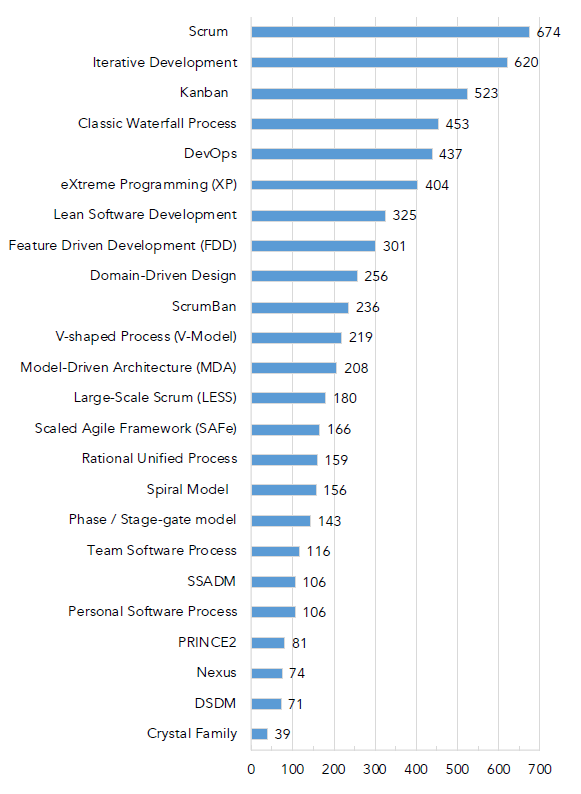
\includegraphics[width=0.7\textwidth]{Bilder/Kapitel-2/VerteilungModelleMethoden.png}
    \caption[Eingesetzte Vorgehensmodelle und Methoden]{Eingesetzte Modelle und Methoden. Mehrfachnennung war möglich. \cite[10]{kuh18}}
    \label{fig:softwareentwicklungsmodelle_und_methoden}
\end{figure}

Die Studienreihe „Status Quo Agile“ der Hochschule Koblenz untersucht regelmäßig den Status Quo der Nutzung agiler Methoden. Für die Studie „Status Quo Agile – 3.~Studie zu Verbreitung und Nutzen agiler Methoden 2016/2017“ \cite{kom17} wurden etwa 1000 Unternehmen aus über 30~Ländern befragt, wobei aber 73\,\% der teilgenommenen Befragten aus Deutschland stammen. 

\pagebreak %%% für Druck

20\,\% der Befragten gaben an nur mit agilen Methoden zu arbeiten (s. Abb.~\ref{fig:einsatz_agiler_methoden}), während 12\,\% nur mit klassischen Methoden arbeiten. Das bedeutet, dass mehr als zwei Drittel der befragten Unternehmen entweder klassische und agile Methoden mixen (Kategorie Hybrid) oder bei einzelnen ausgewählten Prozessen agile Methoden einsetzen (Kategorie Selektiv). In der 4.~Studie der Reihe „Status Quo (Scaled) Agile 2019/20. 4.~Internationale Studie zu Nutzen und Erfolgsfaktoren (skalierter) agiler Ansätze“ \cite{kom20} hat sich im Jahr 2019 an diesem Befund nur wenig verändert. Der Anteil rein klassischer Methoden ist mit 9\,\% der Projekte etwas gesunken, der Anteil der durchgängig agilen Projekte liegt weiterhin bei 20\,\%, die hybriden Projekte konnten mit 43\,\% gegenüber dem nur selektiven Einsatz (28\,\%) etwas zulegen \cite[13]{kom20}.

\begin{figure}[h!]
    \centering
    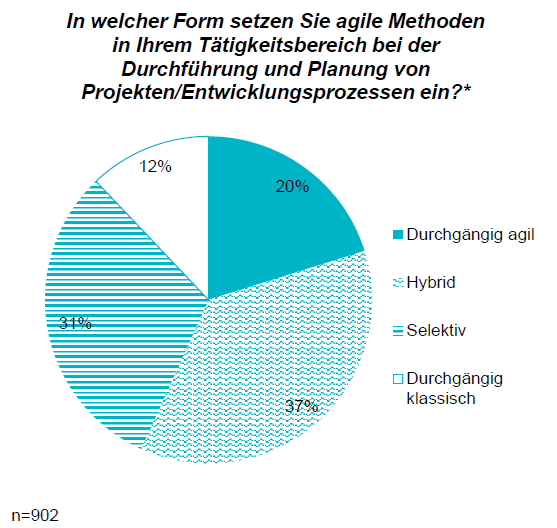
\includegraphics[width=0.7\textwidth]{Bilder/Kapitel-2/EinsatzAgileMethoden.png}
    \caption[Einsatz agiler Methoden bei der Durchführung von Projekten]{Einsatz agiler Methoden bei der Durchführung und Planung von Projekten/Entwicklungsprozessen \cite[15]{kom17}}
    \label{fig:einsatz_agiler_methoden}
\end{figure}

Die Status Quo Agile-Studienreihe hat die Verbreitung agiler Methoden im Blick und fragte daher 2017 auch nach den Gründen, aus denen selektive bzw. hybride Formen – wie aus den vorgegebenen Antwortkategorien hervorgeht: an Stelle komplett agiler Formen – gewählt wurden (Abb.~\ref{fig:gruende_hybrid}). 

%%% Hier kommt Abbildung "fig:gruende_hybrid" eigentlich hin.

Auffällig ist hier, dass anscheinend häufig organisatorische Rahmenbedingungen und institutionelle Zwänge dem reinen agilen Vorgehen im Weg stehen. Vor diesem Hintergrund ist es nicht verwunderlich, dass ein agiles Modell wie Scrum, das deutlich managementfreundlicher als andere agile Modelle ist, sich gegenüber anderen agilen Modellen durchsetzen konnte. In der 4. Studie der Reihe wurde die Frage erneut – allerdings mit etwas abweichenden Antwortkategorien – gestellt \cite[24]{kom20}: Hauptgrund für die Nicht-Wahl eines reinen agilen Ansatzes bleiben die Rahmen\-bedin\-gungen (74\,\%). 

\pagebreak %%% für Druck

\begin{figure}[h!]
	\begin{addmargin*}[0cm]{-\marginparwidth}
		\begin{addmargin*}[0cm]{-\marginparsep}
			\centering
			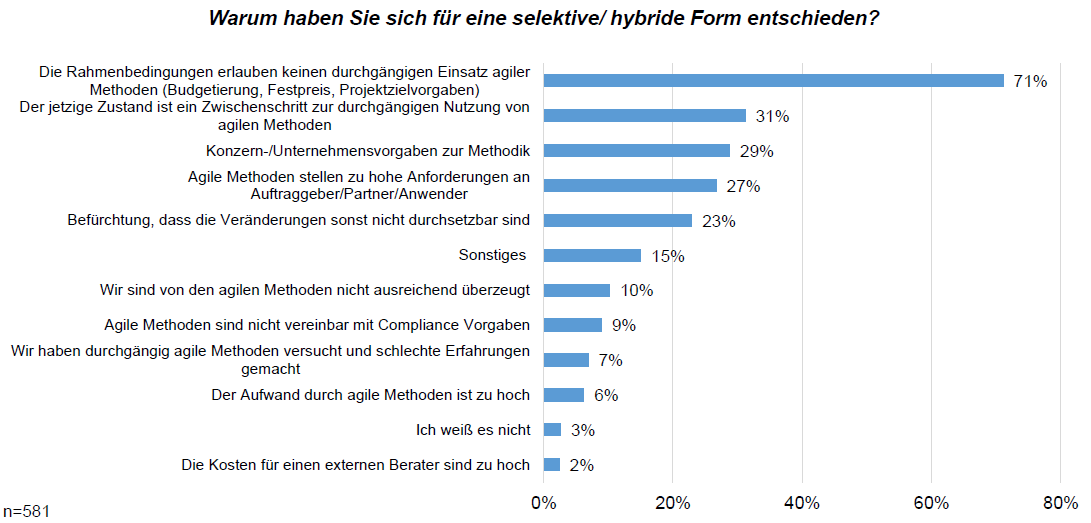
\includegraphics[width=1.25\textwidth]{Bilder/Kapitel-2/GruendeHybrid.png}
			\caption[Gründe für eine selektive/hybride Form]{Gründe für eine selektive/hybride Form. Mehrfachnennung war möglich. \cite[29]{kom17}}
			\label{fig:gruende_hybrid}
		\end{addmargin*}
	\end{addmargin*}
\end{figure}

\begin{figure}[h!]
	\begin{addmargin*}[0cm]{-\marginparwidth}
		\begin{addmargin*}[0cm]{-\marginparsep}
			\centering
			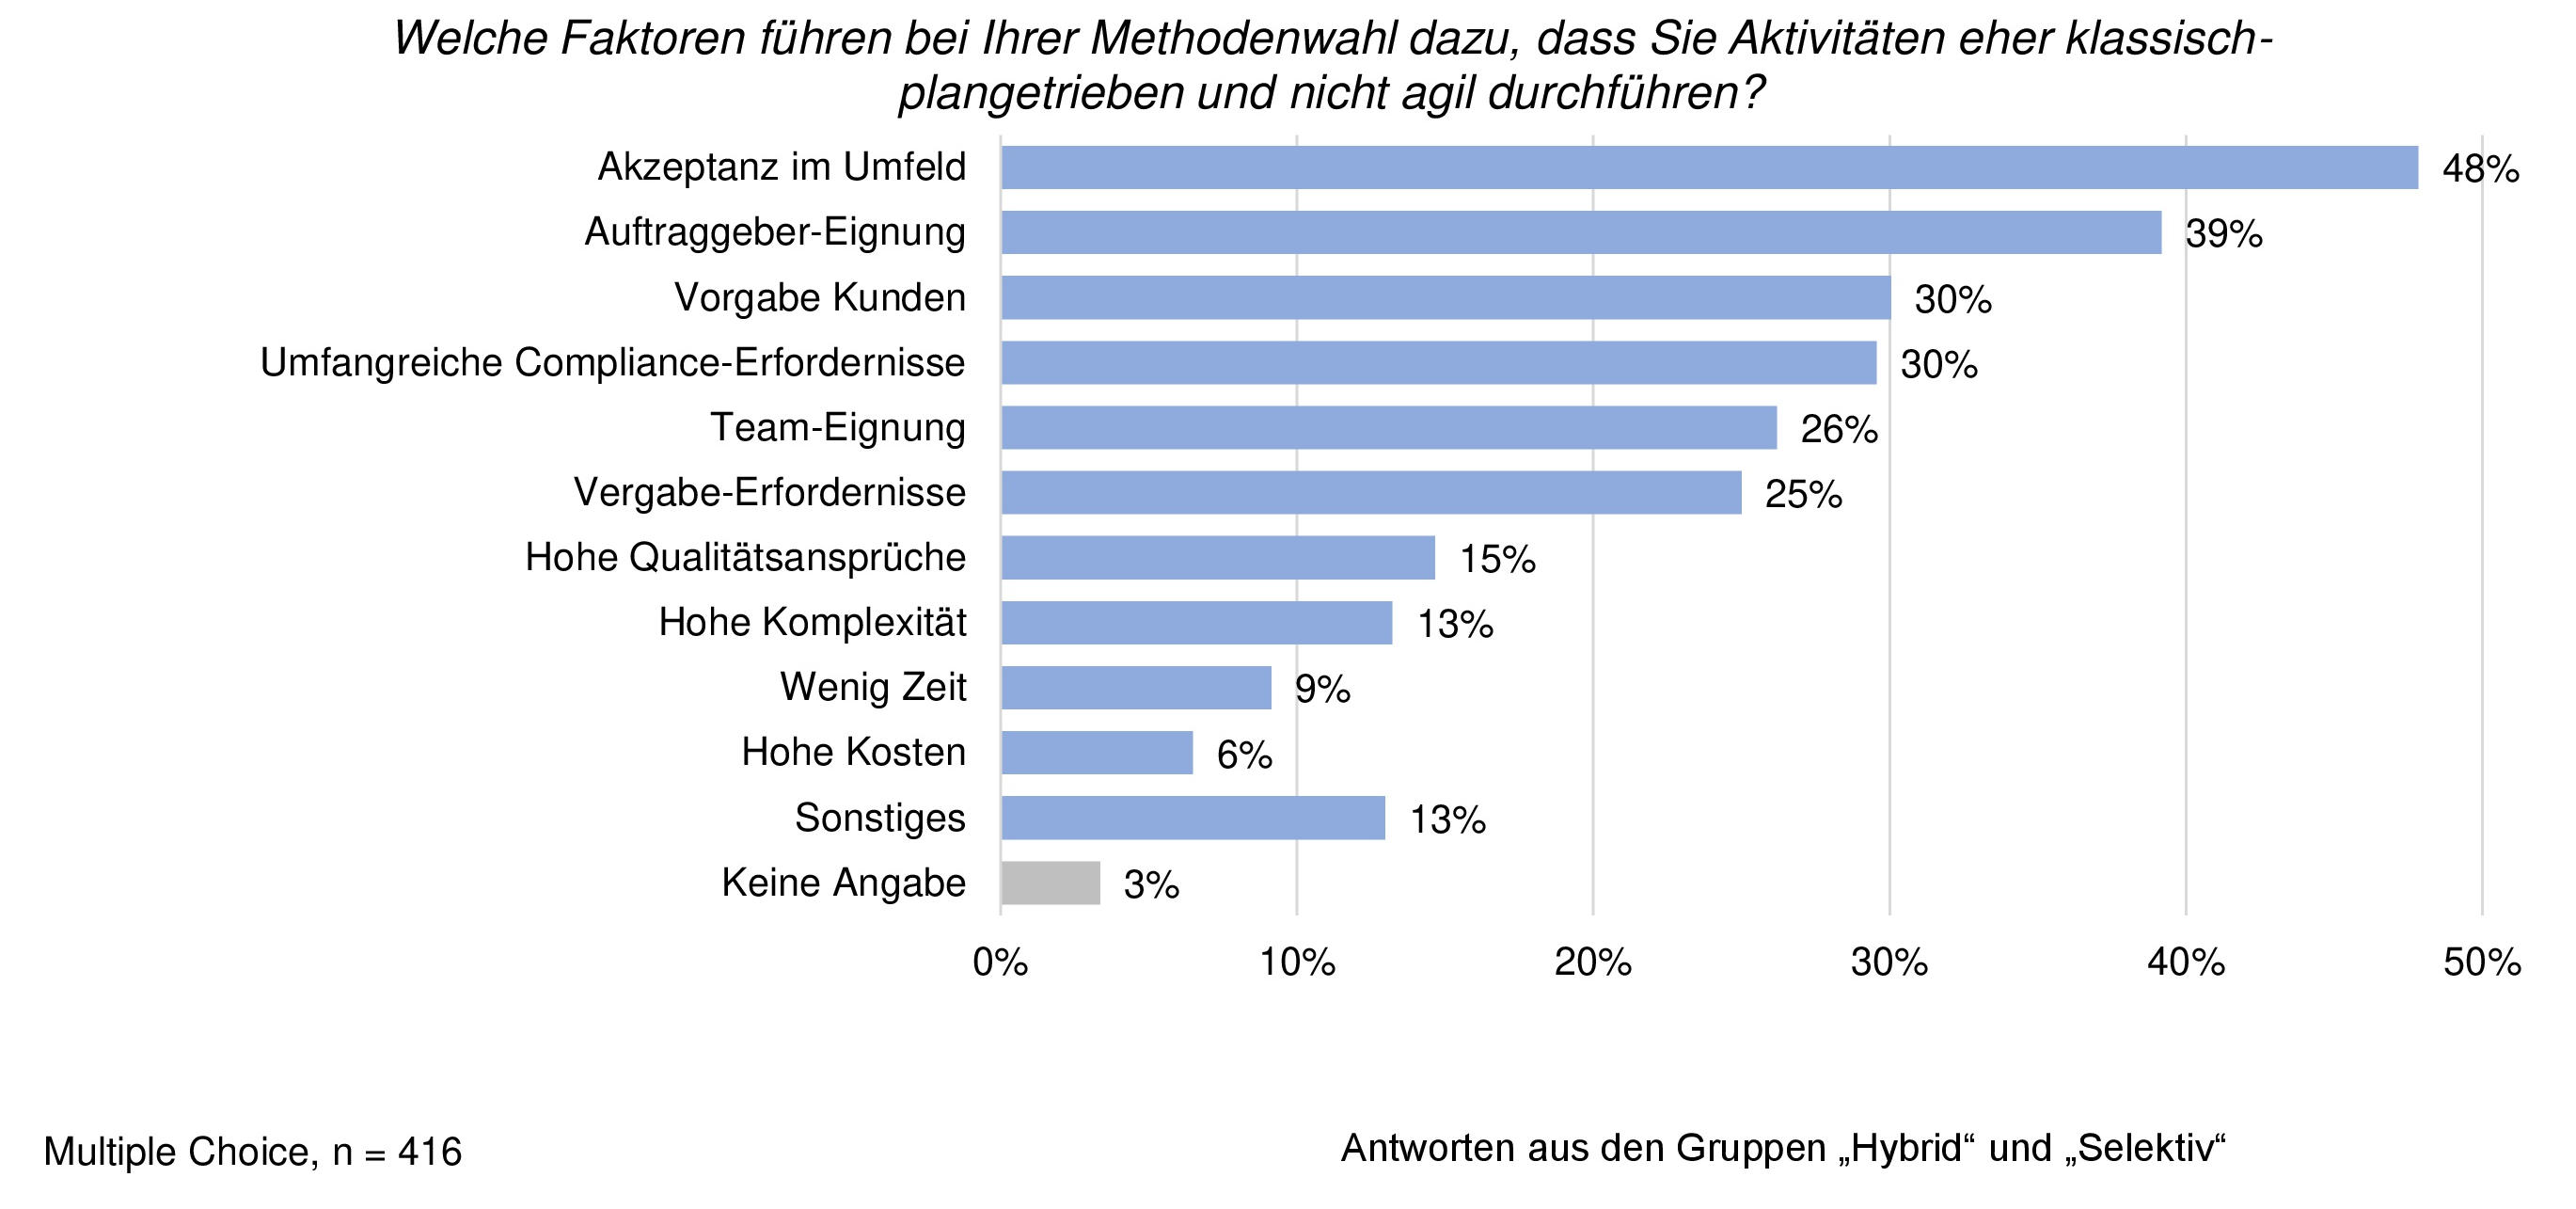
\includegraphics[width=1.25\textwidth]{Bilder/Kapitel-2/GruendeKlassisch.png}
			\caption[Faktoren für die Wahl klassisch-plangetriebener Methoden]{Faktoren für die Wahl klassisch-plangetriebener Methoden. Mehrfachnennung war möglich. \cite[30]{kom20}}
			\label{fig:gruende_klassisch}
		\end{addmargin*}
	\end{addmargin*}
\end{figure}

\pagebreak %%% für Druck

Die 2019er-Studie fragt bei Projekten, die in die Kategorien Hybrid oder Selektiv fallen, außerdem nach den Gründen für die Wahl klassisch-plangetriebener statt agiler Methoden (Abb.~\ref{fig:gruende_klassisch}). Auch hier zeigt sich, dass für die Entscheidung zwischen agilen und plangetriebenen Methoden oft weniger einzelnen Methoden innewohnende Vor- oder Nachteile, sondern vielmehr die verschiedenen Umfeldfaktoren des Softwareentwicklungsprojekts eine Rolle spielen. 

%%% Hier kommt Abbildung "fig:gruende_klassisch" eigentlich hin.

Über Scrum sagen in der 2017er-Studie etwa 55\,\% derjenigen Befragten, die agile Methoden einsetzen, dass es eine zentrale Bedeutung in ihrem Tätigkeitsbereich habe und weitere etwa 25\,\%, dass es neben anderen Methoden in ihrem Tätigkeitsbereich genutzt werde \cite[50]{kom17}\footnote{die Frage lautete: „Welche Bedeutung haben die jeweiligen Methoden für Ihren Bereich?“. Die anderen beiden Antwortkategorien waren „geringe Bedeutung in meinem Tätigkeitsbereich“ und „keine Bedeutung für meinen Tätigkeitsbereich“, siehe \cite[50]{kom17}}. Damit führt Scrum eine Liste von 14 agilen Methoden an, für die die Studie die Bedeutung abfragt. XP liegt mit etwa 10\,\% für „zentrale Bedeutung“ und weiteren 20\,\% für „neben anderen Methoden genutzt“ in dieser Liste auf Platz~6.

Heute werden sie alle irgendwo eingesetzt – die sequentiellen Vorgehensmodelle, die agilen Vorgehensmodelle und vor allem die diversen Ausprägungen dazwischen! Manche Unternehmen versuchen eine gewisse Standardisierung zu erreichen und Projekte nach unternehmenseinheitlichen Vorgehensmodellen durchzuführen. Andere setzen je nach Projekt unterschiedliche Modelle ein. Es ist dabei sehr üblich die Grundform eines Vorgehensmodells spezifisch an das konkrete Projekt oder an übergeordnete Regeln des Unternehmens anzupassen. Die Status Quo Agile-Studie 2017 hat bei Projekten, die Scrum einsetzen, erhoben, inwieweit sich diese von den Vorgaben von Scrum entfernen und auf Grundlage von Scrum ihr eigenes unternehmens\-spezifisches Vorgehensmodell entwickeln: So setzen 11\,\% der Befragten Scrum ohne die Rolle des Scrum Master ein, in weiteren 19\,\% der Projekte agiert der Scrum Master eher wie ein (klassischer) Projektleiter, und 20\,\% der Projekte setzen einen Scrum Master und einen Projektleiter gleichzeitig ein \cite[99]{kom17}. Insofern halten sich nur die Hälfte der befragten Projekte an die in Scrum definierte Rollenausgestaltung des Scrum Master. Ein ähnliches Abweichen vom Grundmodell ist bei der Rolle des Product Owner zu beobachten: 13\,\% der Projekte haben gar keinen Product Owner bzw. lassen die Rolle von einem Mitglied des Entwicklungsteams übernehmen, und in 35\,\% der Projekte definiert der Product Owner die Sprint-Ziele \cite[100]{kom17}, obwohl Scrum hier explizit die gemeinsame Abstimmung zwischen Product Owner und Entwicklungsteam fordert.

\minisec{Fazit}

Sie haben im Laufe des Kapitels verschiedene Kriterien kennengelernt, anhand derer man Vorgehensmodelle unterscheiden kann. Die größten Unterschiede bestehen in den Strategien der Vorgehensmodelle mit neuen oder veränderten Anforderungen umzugehen. Warum ist das so? In einer idealen Welt, in der man für die Entwicklung eines Softwareprodukts unendlich viel Zeit und Geld hätte, alle Anforderungen unmissverständlich benennen könnte und wüsste, dass sich diese Anforderungen niemals ändern würden; in dieser Welt würde man zu Beginn eines Projekts alle Anforderungen detailliert aufschreiben, denn je umfänglicher man zu Beginn über die gewünschte Funktionalität Bescheid weiß, desto zielgerichteter und effizienter kann die Software entwickelt werden. Nur ist das leider unrealistisch. Daher muss jedes konkrete Softwareentwicklungsprojekt in irgendeiner Weise den Spagat schaffen notwendige Änderungen – im Übrigen nicht nur bezogen auf die Anforderungen – im Laufe des Projekts vornehmen zu können und gleichzeitig in der Lage sein das Zeit- und Kostenbudget möglichst einzuhalten, wofür in der Regel die Kontrolle des Projektfortschritts notwendig ist. Die verschiedenen Vorgehensmodelle verfolgen dafür unterschiedliche Strategien. Mit dem flexiblen Reagieren auf Änderungen haben sequentiell orientierte Entwicklungsprojekte die meisten Schwierigkeiten. Die Messung des Projektfortschritts stellt am häufigsten agile Projekte vor Probleme. Es ist daher nicht erstaunlich, dass verschiedene hybride Vorgehensmodelle publiziert werden, die versuchen – und in der Regel auch für sich in Anspruch nehmen es geschafft zu haben – die als sinnvoll erachteten Methoden aus klassischen und agilen Modellen optimal zu vereinen. Mit diesen hybriden Modellen werden wir uns nicht beschäftigen, da uns keines bekannt ist, das aktuell einen größeren Verbreitungsgrad erreicht hätte. Wie auch aus den oben gezeigten Grafiken deutlich wird, gestalten sich Unternehmen oder Projekte sowieso häufig ihre eigenen hybriden Modelle, indem sie zum Beispiel eigentlich agile Modelle um klassische Methoden zum Beispiel zu Projektplanung, Controlling oder Dokumentation erweitern oder in eigentlich sequentielle Modelle agile Elemente zum Beispiel für den Umgang mit Änderungen oder eine andere Art des Testens einbauen.\footnote{\cite{kuh19} werten auf Grundlage der HELENA-Daten \cite{kuh18} hybrides Vorgehen in europäischen Softwareentwicklungsprojekten aus. Der Artikel enthält eine Übersichtstabelle (S.~24~f.) mit Informationen, welche klassischen und welche agilen Methoden von den befragten Projekten kombiniert wurden.}

Ein noch immer heftig diskutiertes Thema im Kontext der Vorgehensmodelle ist die Skalierung von agilen Modellen. Agile Ansätze sind ursprünglich für kleine bis mittlere Teamgrößen gedacht, bei denen die Teammitglieder am selben Ort arbeiten. Diskutiert wird, ob und wie agile Ansätze auch für große und sehr große Entwicklungsteams oder regional verteilt arbeitende Teams sinnvoll eingesetzt werden können. Zu diesem Zweck wurden verschiedene Modelle publiziert. Drei der bekannteren sind das Scaled Agile Framework (SAFe) von Dean Leffingwell, das Agile Scaling Model (ASM) von Scott Ambler und Large-Scale Scrum (LeSS) von Bas Vodde and Craig Larman.\footnote{Weiterführende Informationen zur Skalierung agiler Ansätze und den genannten Modellen bei \cite[104 \psqq]{som18}, \cite[95 \psqq]{kom20} und \cite[41 \psqq]{amb11}.}

Im Umfeld der Vorgehensmodelle auch eher neu (etwa seit den 2010er Jahren) und doch gleichzeitig in gewisser Weise auch sehr alt – weil unter dem Aspekt Wartung schon in manchen sequentiellen Modellen vorhanden – ist die Ausweitung des Blickfelds der Softwareentwicklung in Richtung Softwarebetrieb. Dies ist insbesondere im Rahmen agiler Softwareentwicklung relevant, da Versionen der Software sehr häufig schon produktiv eingesetzt werden, während das Entwicklungsprojekt noch läuft und das Softwareprodukt kontinuierlich weiterentwickelt. Ansätze wie DevOps  
%\sttpkapitelverweis{DevOps}{Kap.~\ref{sec:Kap-x.y}}
betonen daher die Notwendigkeit, Prozesse der Softwareentwicklung und Prozesse des Softwarebetriebs viel enger miteinander zu verknüpfen – auch personaltechnisch. 

Jenseits der Fragen, ob Softwareentwicklung mehr oder weniger Prozesse benötigt, mehr oder weniger Dokumentationen zum Produkt erzeugen muss, sequentieller oder agiler erfolgen sollte; einer der wichtigsten Faktoren für eine erfolgreiche Software\-entwicklung bleibt das Entwicklungsteam. So mag oftmals die Wahl der Methoden und Vorgehensmodelle mehr von der Qualifikation der beteiligten Menschen abhängen als von den Charakteristika des Projekts. Die Vorgehensmodelle sind wichtig und hilfreich, aber mit einem unmotivierten Team entwickelt man mit jedem Vorgehensmodell schlechte Software - oder auch gar keine. Insofern gilt auch heute noch die mehr als dreißig Jahre alte Analyse von Watts Humphrey, der über viele Jahre einer der zentralen Akteure im Bereich der (klassischen) Software\-prozess\-verbesserung war: Es bedarf in jedem Softwareentwicklungsprojekt immer wieder der Abwägung zwischen dem „individual need for flexibility and the organizational need for standards and consistency“. Und dabei ist in jedem Fall zu berücksichtigen: 

\vspace{3mm} %%% für Druck

\sttpzitat{„Since software projects have differences, their software engineering processes must have differences as well. [...] In the absence of a universal software engineering process, organizations and projects must define processes that meet their own unique needs.“ Humphrey 1989, zitiert nach \cite[685]{sha11}}{}

\vspace{3mm} %%% für Druck

Letztendlich muss jedes Softwareentwicklungsprojekt für sich selbst herausfinden, nach welchem Vorgehen die Erstellung qualitativ hochwertiger Softwareprodukte in gegebenen Zeit-, Personal- und Kostenbudgets sowie bei gegebenen Rahmenbedingungen am besten gelingt.